%------------------------------------------------------------------------------
% ILLUMINE overview --- Journal of Synchrotron Radiation (IUCr)
% Current IUCr submission class for all journals, including JSR:
%   \documentclass{iucrjournals}
%   https://journals.iucr.org/s/services/latexstyle.html
%   https://journals.iucr.org/services/latexstyle.html
% Legacy JSR-only invocation (older iucr.cls) was:
%   \documentclass[preprint]{iucr}
%   \journalcode{S}
% Strawman article type: Feature article (TBD vs research paper).
% This file is a coordination skeleton for the 18 August 2026 All Hands
% (T-96). Highlight cells are placeholders; do not treat them as claims.
%------------------------------------------------------------------------------

\documentclass{iucrjournals}

\usepackage{booktabs}
\usepackage{tabularx}
\usepackage{tikz}
\usetikzlibrary{arrows.meta,positioning,fit,calc}

\title{ILLUMINE at year three: edge-to-HPC analysis, decision support, and a
Bluesky steering layer}

% Full collaboration list: edit authors.tex (one line per person).
% !TeX root = ./main.tex
%------------------------------------------------------------------------------
% ILLUMINE author list (IUCr / JSR)
% Included from main.tex before \begin{document}.
%
% How to add someone (one line):
%   \IllumineAuthor{a}{Given Family}
%   \IllumineAuthor{a,d}{Given Family}[email@lab.gov]
%   \IllumineAuthor{a}{Given Family}[email@lab.gov][0000-0000-0000-0000]
% Corresponding author (blue envelope icon):
%   \IllumineCorresponding{a}{Given Family}[email@lab.gov][ORCID]
%
% Affiliation letters are defined at the bottom. Reuse letters; do not
% invent a new letter for a second person at the same lab.
%
% Starter names = 2023 proposal named Co-Is (LAB 23-3030 cover) plus
% F. Poitevin for this paper. All Hands speakers are not auto-authors.
% Order: corresponding first, then by laboratory (proposal order),
% alphabetical within a lab. Confirm spelling, emails, ORCIDs, and
% whether 2026 staff who were not Co-Is should be added.
%------------------------------------------------------------------------------

\NewDocumentCommand{\IllumineAuthor}{m m o o}{%
  \author[#1]{#2%
    \IfValueT{#3}{\IUCrEmaillink{#3}}%
    \IfValueT{#4}{\IUCrOrcidlink{#4}}%
  }%
}
\NewDocumentCommand{\IllumineCorresponding}{m m o o}{%
  \author[#1]{#2%
    \IfValueTF{#3}{\IUCrCemaillink{#3}}{\IUCrAufn{Corresponding author.}}%
    \IfValueT{#4}{\IUCrOrcidlink{#4}}%
  }%
}

% --- SLAC / LCLS (a) and SSRL (b) -----------------------------------------
\IllumineCorresponding{a}{Jana Thayer}[jana@slac.stanford.edu]
\IllumineAuthor{a}{Ryan Herbst}
\IllumineAuthor{a}{Fr\'ed\'eric Poitevin}[frederic.poitevin@stanford.edu][0000-0002-3181-8652]
\IllumineAuthor{a}{Chun Hong Yoon}
\IllumineAuthor{b}{Vivek Thampy}
% \IllumineAuthor{b}{Apurva Mehta} % SSRL facility co-lead in management plan; not a named Co-I on the cover

% --- BNL / NSLS-II (d) ----------------------------------------------------
\IllumineAuthor{d}{Daniel Allan}
\IllumineAuthor{d}{Andi Barbour}
\IllumineAuthor{d}{Stuart Campbell}
\IllumineAuthor{d}{Thomas Caswell}
\IllumineAuthor{d}{Natalie Isenberg}
\IllumineAuthor{d}{Phillip Maffettone}
\IllumineAuthor{d}{Daniel Olds}
\IllumineAuthor{d}{Max Rakitin}
\IllumineAuthor{d}{Nathan Urban}

% --- ANL / APS (c) --------------------------------------------------------
\IllumineAuthor{c}{Franck Cappello}
\IllumineAuthor{c}{Robert Underwood}
\IllumineAuthor{c}{Ian Foster}
\IllumineAuthor{c}{Antonino Miceli}
\IllumineAuthor{c}{Nicholas Schwarz}

% --- LBNL / ALS (e) -------------------------------------------------------
\IllumineAuthor{e}{Alexander Hexemer}
\IllumineAuthor{e}{Dylan McReynolds}
\IllumineAuthor{e}{Wiebke K{\"o}pp}
\IllumineAuthor{e}{Xiaoya Chong}

% --- ORNL / SNS+HFIR (f) --------------------------------------------------
% Cover page: Jonathon Taylor; budget Co-PI line: Jonathan Taylor.
\IllumineAuthor{f}{Jonathan Taylor}

% Copy this line for 2026 additions (uncomment and fill):
% \IllumineAuthor{a}{Given Family}[email][0000-0000-0000-0000]

% --- Affiliations (authblk letters) ---------------------------------------
\affil[a]{Linac Coherent Light Source, SLAC National Accelerator Laboratory, Menlo Park, CA 94025, USA}
\affil[b]{Stanford Synchrotron Radiation Lightsource, SLAC National Accelerator Laboratory, Menlo Park, CA 94025, USA}
\affil[c]{Argonne National Laboratory, Lemont, IL 60439, USA}
\affil[d]{National Synchrotron Light Source II, Brookhaven National Laboratory, Upton, NY 11973, USA}
\affil[e]{Advanced Light Source, Lawrence Berkeley National Laboratory, Berkeley, CA 94720, USA}
\affil[f]{Oak Ridge National Laboratory, Oak Ridge, TN 37831, USA}


\begin{document}
\maketitle

\begin{abstract}
ILLUMINE (\textit{Intelligent Learning for Light Source and Neutron Source User
Measurements Including Navigation and Experiment Steering}) is a five-year,
multi-facility effort to put actionable information in front of experimenters
at detector rates and to close the loop from reduction to the next measurement
on a shared Bluesky-based framework. The 2023 diagnosis still holds: facilities
need a fast inner loop (edge reduction to controls) and a slower outer loop
(HPC analysis and decision support into a steering layer), as a first step
toward DOE Integrated Research Infrastructure. This article is a mid-term
snapshot, written in years~3--4 of award LAB~23-3030, not a restatement of the
proposal abstract. We report what has shipped against the three original aims
--- real-time analysis at the edge and edge-to-HPC, workflow monitoring and
decision support, and an autonomous steering toolbox --- what has remained
local to a beamline, and where integration is still the hard part. A short 2026
addendum distinguishes the proposal's ``Decision Agent'' modules (pluggable
reducers and choosers in a Bluesky pipeline) from language-model copilots that
sit on top of that stack. The intended length is about 3500~words, one updated
architecture figure, and one cross-facility evidence table keyed to quarterly
demos.
\end{abstract}

\begin{synopsis}
A mid-term snapshot of ILLUMINE: what the three 2023 aims have delivered at
the edge, in decision support, and in Bluesky steering, and what ``agent''
should mean in 2026.
\end{synopsis}

\keywords{
synchrotron radiation;
X-ray free-electron laser;
real-time analysis;
edge computing;
decision support;
Bluesky;
experiment steering;
autonomous experiments;
ILLUMINE
}

%------------------------------------------------------------------------------
\section{Introduction}
\label{sec:intro}

User facilities still face a rate mismatch. Detectors outrun the analysis that
would tell an experimenter whether the last measurement was worth keeping, and
steering --- when it exists --- is often a local script rather than a shared
layer. ILLUMINE was funded to close that gap across light sources and neutron
sources: put reduced, science-relevant information on the same timescale as
acquisition, and couple it to the next control action through a common
framework rather than a one-off stack per hutch \cite{illumine2023}.

The original claim was architectural, not a catalogue of widgets. Figure~1 of
the 2023 proposal (redrawn here as Fig.~\ref{fig:loops}) separates an inner
\textbf{fast} loop --- Aim~1 reduction feeding controls --- from an outer
\textbf{slow} loop --- Aim~1 HPC products plus Aim~2 recommendations feeding
Aim~3 Bluesky plans. That figure is still the right spine. The work of this
paper is to colour the boxes with what is live, what is prototype, and what is
still a slide, not to invent a new architecture unless Fig.~\ref{fig:loops} is
wrong.

We are in years~3--4 of a plan that runs from 1~September 2023 to 31~August
2028 (PI Jana Thayer; collaborating laboratories SLAC, ANL, ORNL, BNL, and
LBNL). Fully self-driving beamlines were the horizon in 2023, not the year-3
requirement; a human in the loop was already in the proposal. Language-model
copilots were not. Section~\ref{sec:agents} therefore treats 2026 agent
language as an addendum on top of Fig.~\ref{fig:loops}, not as a fourth aim
and not as a rename of the 2023 Decision Agent.

This is not an LCLS-only autoMFX paper, not a 40-author brochure, and not a
new proposal. Companion instrument papers can carry beamline-specific methods.
The consortium paper should be judged on whether the three aims compose.

\begin{figure}[t]
\centering
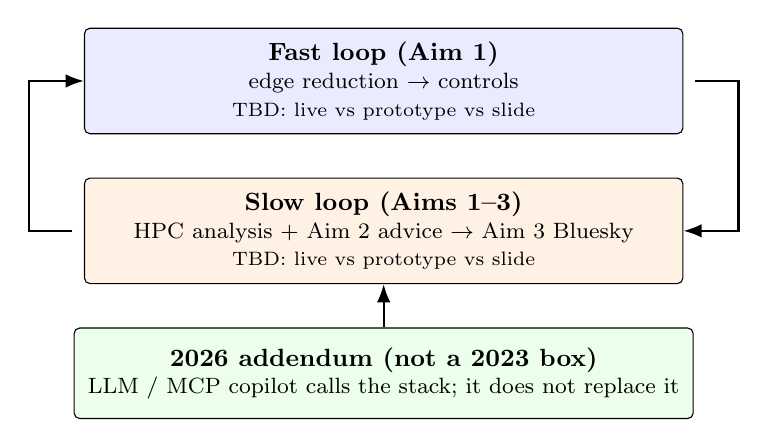
\begin{tikzpicture}[
  font=\small,
  box/.style={draw, rounded corners=2pt, align=center, inner sep=5pt, minimum height=1.15cm},
  flow/.style={-{Latex}, thick},
]
  \node[box, fill=blue!8, minimum width=7.6cm] (fast) {%
    \textbf{Fast loop (Aim~1)}\\[-1pt]
    {\footnotesize edge reduction $\rightarrow$ controls}\\[-1pt]
    {\scriptsize TBD: live vs prototype vs slide}};
  \node[box, fill=orange!10, minimum width=7.6cm, below=0.55cm of fast] (slow) {%
    \textbf{Slow loop (Aims~1--3)}\\[-1pt]
    {\footnotesize HPC analysis + Aim~2 advice $\rightarrow$ Aim~3 Bluesky}\\[-1pt]
    {\scriptsize TBD: live vs prototype vs slide}};
  \node[box, fill=green!8, minimum width=7.6cm, below=0.55cm of slow] (llm) {%
    \textbf{2026 addendum (not a 2023 box)}\\[-1pt]
    {\footnotesize LLM / MCP copilot calls the stack; it does not replace it}};
  \draw[flow] (fast.east) ++(0.15,0) coordinate (e1) -- ++(0.55,0) |- (slow.east);
  \draw[flow] (slow.west) ++(-0.15,0) -- ++(-0.55,0) |- (fast.west);
  \draw[flow] (llm.north) -- (slow.south);
\end{tikzpicture}
\caption{ILLUMINE control loops, after proposal Fig.~1. Inner loop: Aim~1
reduction on a timescale that can touch controls. Outer loop: Aim~1 HPC
products and Aim~2 decision support into Aim~3 Bluesky plans. Language-model
agents (bottom) are a 2026 control plane on top of that figure, not a
replacement for reduction, Gaussian-process/RL choosers, or Bluesky.
\textit{Update owner TBD:} recolour boxes to live / prototype / not yet.}
\label{fig:loops}
\end{figure}

%------------------------------------------------------------------------------

\section{Aim 1 --- real-time analysis at the edge and edge-to-HPC}
\label{sec:aim1}

\textit{Strawman owners: Cappello, with Yoon (calibration, Bragg finder),
Herbst/Miceli (FPGA), Foster/Schwarz (HPC retraining). $\sim$700 words.}

Aim~1 is the inner loop plus the HPC path that the outer loop still needs.
Applications named in 2023 were ptychography, crystallography, and tomography,
with diffraction workflows alongside. Sub-deliverables included ultrafast
calibration (including a crystallography demonstration); a Bragg-peak finder
that runs on \emph{uncalibrated} images for FEL, synchrotron, and neutron
sources, with closed loop at LCLS, APS, and HFIR; transformer-based lossy
reduction and compact models on FPGAs; file-based and streaming HPC workflows;
and model re-training with a shared repository.

Edge and FPGA work does not retire HPC, and HPC does not give millisecond
steering. Both timescales remain in Fig.~\ref{fig:loops}. The section should
say what is streaming versus file-based, what is on the detector path versus
after the file, and which science metric (Bragg quality, ptycho reconstruction,
tomography artifact) the reducer actually sees.

\textit{Placeholders from the August 2026 All Hands, not an outline:} FPGA
status; compression comparisons; streaming and Tiled. LCLS crystallography
content belongs here and in Aim~3, not as the whole consortium story. Do not
quote Run~26 downtime percentages without facility operations.

\subsection{Compression}
\textit{Strawman owners: Cappello and Underwood $\sim$1200 words. for this subsection}

Why compression for light sources.

What has been explored as part of the Illumine
In the past, we have explored several compression approaches for reducing the massive data movement and storage requirements of light source experiments with Advanced Photon Source (APS). 
One major outcome is lsCOMP, a GPU-based compression framework specifically designed for the irregular unsigned integer data generated by APS applications. 
Unlike conventional compressors that are often designed for general-purpose byte streams or smooth scientific data, lsCOMP supports configurable lossless and lossy compression through adaptive scalar quantization, selective pooling, and zero-bit elimination. 
These operations are integrated into a highly optimized single-GPU-kernel design, allowing lsCOMP to achieve compression throughput of hundreds of GB/s on a single NVIDIA A100 GPU while maintaining high compression ratios and application-level data quality. 
The resulting tool has been open-sourced and published at SC 2025 (DOI: 10.1145/3712285.3759814; Code: https://github.com/szcompressor/lsCOMP).
Beyond GPU compression, we have explored how compression can be integrated more deeply into the APS end-to-end light-source data path. 
In particular, light-source workflows involve heterogeneous instruments, computing platforms, networks, and storage systems with substantially different resource and bandwidth constraints. 
This makes compression a system-level optimization problem rather than simply a standalone compression-kernel problem: an approach that performs well at one stage may not provide the best overall performance when data must traverse the complete workflow.
We have also explored learning-assisted compression to exploit redundancy that is difficult for conventional numerical compressors to capture. 
Light source datasets can exhibit complex correlations across measurements, spatial regions, and time, creating opportunities for learned prediction to reduce the amount of information that must be explicitly encoded. 
However, these correlations vary considerably across experiments and scientific applications, making it challenging to achieve high prediction accuracy, user-acceptable inference overhead, and reliable reconstruction simultaneously. 
Together, these explorations highlight the need to co-design compression algorithms with the characteristics of light source data and the systems through which those data move.


What is next for this work.

Note Lessons Learned from this

\subsection{Edge Computing}



%------------------------------------------------------------------------------
\section{Aim 2 --- workflow monitoring and decision support}
\label{sec:aim2}

\textit{Strawman owners: Urban / Isenberg. $\sim$500 words.}

Aim~2 was never ``remove the scientist.'' The 2023 text already wanted a human
in the loop: reinforcement learning for data collection in Bluesky; high-dimensional
search and visualization; clustering and classification (UMAP/SOM); and
decision support under uncertainty (hierarchical Gaussian processes, Bayesian
optimization). Science examples in the proposal narrative included additive
manufacturing (ALS, APS, LCLS, SSRL, NSLS-II), protein crystallography and
ultrafast dynamics at LCLS and SSRL, neutron sample positioning and acquisition
at SNS/HFIR, and operational/logistics automation.

Steering that does not see a science quality metric is just faster knobs. This
section should name the intent function (or the human-facing surrogate) and
where uncertainty is shown, not only that a scan ran unattended.

\textit{Placeholders:} BLOP and related Bayesian loop tools; powder
automation; auto phase detection; ROI / BORA; facility-specific decision UIs.

%------------------------------------------------------------------------------
\section{Aim 3 --- Bluesky steering framework}
\label{sec:aim3}

\textit{Strawman owners: Campbell, with Allan, Maffettone, Caswell, Rakitin,
Barbour, Olds. $\sim$500 words.}

Aim~3 is the shared loop, not a new control system. The four steps in the
proposal are reduce, decide the next action, encode it to controls, and
collect. Two timescales sit inside that loop: faster than a measurement
(instrument optimization) and commensurate with a measurement (sequence
planning). Interoperation was specified with the Queue Server, workflow
systems, and parameterized similar measurements (for example powder). The UI
was specified to show the live experiment, agent state, history, queued plans,
and hyper-parameters \cite{allan2019bluesky}.

Bluesky was the reference implementation \emph{because} pieces can be adopted
without replacing a beamline. This paper should score that interop claim, not
assume a single stack won.

The 2023 ``Agents'' are pluggable modules in this pipeline --- local or
facility/HPC --- that consume reduced data and emit the next measurement or
control directive. Gaussian-process fly-scan demos at NSLS-II already existed
when the proposal was written. They are not language models.

\textit{Placeholders:} Bluesky/Tiled status; LCLS MFX photon-beam tuning and
operator-facing skills as one Aim~3 + Aim~1 crystallography cell.

%------------------------------------------------------------------------------
\section{Cross-facility evidence}
\label{sec:evidence}

\textit{One named owner per facility; $\sim$400 words plus Table~\ref{tab:m4}.}

Quarterly facility demonstrations (proposal milestones M4-1 through M4-7) are
the natural evidence cadence. Table~\ref{tab:m4} should reuse that cadence
rather than invent a new scorecard. Empty cells are more useful than optimistic
prose.

\begin{table}[t]
\centering
\caption{Cross-facility snapshot keyed to ILLUMINE quarterly demos (M4).
Fill at All Hands; ``last demonstrated'' beats ``planned.''}
\label{tab:m4}
\begin{tabular}{lllp{4.4cm}}
\toprule
Facility & Owner & Last demonstrated & Notes (live / prototype / local-only) \\
\midrule
LCLS (SLAC) & TBD & TBD & MFX / crystallography cell \\
APS (ANL) & Schwarz & TBD & \\
NSLS-II (BNL) & Campbell & TBD & \\
ALS (LBNL) & Hexemer & TBD & \\
SSRL (SLAC) & Thampy / Mehta & TBD & \\
SNS / HFIR (ORNL) & Taylor & TBD & \\
\bottomrule
\end{tabular}
\end{table}

%------------------------------------------------------------------------------
\section{Lessons: transfer versus local}
\label{sec:lessons}

\textit{Mixed authorship. $\sim$350 words.}

The 2023 proposal already named the failure mode: Aims~1--3 can mature
separately while the user still stitches them by hand (\S2.7 of the proposal).
The paper should score integration, not only widgets.

A second lesson was also in the proposal (\S2.5): the goal is interoperation,
not replacement of beamline stacks. A third is timescale honesty: the fast and
slow loops both exist. A fourth is that human-in-the-loop was the year-3
design point. A fifth is the science-versus-engineering metric: if Aim~2 cannot
see Aim~1's Bragg / ptycho / tomography quality, the outer loop is optimizing
the wrong thing.

%------------------------------------------------------------------------------
\section{What ``agent'' means in 2026}
\label{sec:agents}

\textit{Strawman owners: Poitevin, with Max/Cong/Xiaoya and other Day-2 MCP
discussants. $\sim$350 words. This section is new relative to the 2023 text.}

Two different objects now share a word.

The 2023 \textbf{Decision Agent} / Bluesky Agent is a module that consumes
reduced data and emits the next measurement or control directive. It may be a
Gaussian process, an RL policy, a classical optimizer, or a rule. It lives
inside Fig.~\ref{fig:loops}.

A 2026 \textbf{language-model agent} is an operator-facing control plane: it
calls Aim~1--3 tools (plans, Tiled, process variables, analysis jobs) in
natural language, with traces and an abort path. LCLS hutch-copilot work and
MCP-versus-skills discussions sit here. These agents do not replace reduction,
GP/RL choosers, or Bluesky. If Genesis or American Science Cloud appear, they
are infrastructure around that control plane, not a fourth scientific aim
unless the corresponding author decides otherwise.

Collapsing the two uses of ``agent'' would make the consortium paper both
historically false and technically unclear.

%------------------------------------------------------------------------------
\section{Outlook: years 4--5}
\label{sec:outlook}

\textit{Strawman owner: Thayer. $\sim$200 words.}

Year~5 in the 2023 plan is a released framework and libraries, not a promise
that this paper can already make. A reasonable snapshot path is a complete
draft by the end of October 2026 and an arXiv posting in December 2026 if the
JSR methods bar is too high for a consortium note; JSR remains the journal
target of this Overleaf project. The next twelve months should be stated as
integration milestones against Table~\ref{tab:m4}, not as new aims.

%------------------------------------------------------------------------------
\begin{acknowledgements}
We thank the ILLUMINE collaboration and the August 2026 All Hands participants
for discussion of scope, section ownership, and evidence. Facility and aim
leads are listed in the author footnote pending the agreed author list.
\end{acknowledgements}

\begin{funding}
ILLUMINE is supported by the U.S. Department of Energy, Office of Science,
Basic Energy Sciences, under award LAB~23-3030 (PI J.~Thayer; period
2023-09-01 to 2028-08-31). SLAC National Accelerator Laboratory is operated by
Stanford University for the U.S.\ DOE under contract DE-AC02-76SF00515.
Additional facility operating contracts to be confirmed by each laboratory.
\end{funding}

\ConflictsOfInterest{The authors declare no conflicts of interest.}

\DataAvailability{No new datasets are reported in this coordination draft.
Code, demo records, and figure sources for the submitted article will be
linked on acceptance or stated as available on request, matching each
facility's data policy.}

\section*{Author contributions}
Coordination draft: J.~Thayer (corresponding, TBD), F.~Poitevin (skeleton and
JSR Overleaf project). Section owners: Aim~1 Cappello \textit{et al.}; Aim~2
Urban / Isenberg; Aim~3 Campbell \textit{et al.}; Table~\ref{tab:m4} one name
per facility; Fig.~\ref{fig:loops} update owner TBD. CRediT roles to be
completed with the agreed author list.

\bibliography{references}

\end{document}
